\section{Evaluation}

Provide an introductory paragraph that summarizes what's in this section: a list of runs/experiments intended to test your implementation and ideas. Describe each of these experiments in a few words/a sentence.

\subsection{Computational platform and Software Environment}

What machine did you run your tests on? What was the processor, its clock rate (GHz), size of L1/L2/L3 cache, how much memory (DRAM), what OS?

What compiler did you use, what compilation flags?

\subsection{Methodology}
\label{sec:methodology}

Describe the procedures you use to test your system.

Performance metrics: describe exactly what metrics you employ to measure performance. It might be elapsed time from instrumentation code you added around the main computational code. Later in the term, it may be something else.

Experimental design: did you run tests over a set of prescribed problem sizes? If so, what were they?

\subsection{Experiment 1}

Describe the experiment in a few sentences: what question are you trying to answer, what problem sizes/etc did you use (it's ok to make reference back to Sec.~\ref{sec:methodology} so you don't have to repeat a lot of details. 

Present the results of your experiment using either tabular forms of information, such as in Table~\ref{tab:MyTable1}, or using charts and graphs as in Fig.~\ref{fig:MyPlot1}.

\begin{table}[t!]
    \centering
    \begin{tabular}{c c c}
        Problem Size (N) & Ideal runtime (sec) & Actual runtime (sec) \\
        \hline 
        1 & 1 & 1 \\
        2 & 0.5 & 0.75 \\
        4 & 0.25 & 0.56 \\
        8 & 0.12 & 0.42 \\
        16 & 0.06 & 0.31 
    \end{tabular}
    \caption{Comparison of actual and ideal runtimes for different problem sizes. The actual runtime does not equal ideal runtime in this configuration.}
    \label{tab:MyTable1}
\end{table}

\begin{figure}
    \centering
    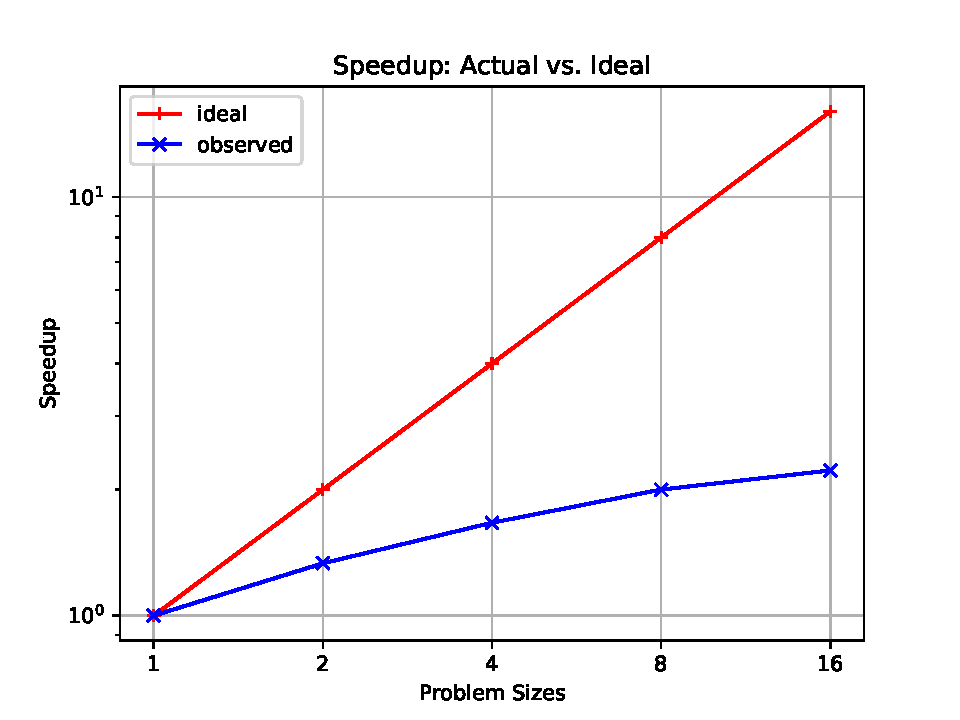
\includegraphics[width=0.45\textwidth]{Figure_1.pdf}
    \caption{Comparison of actual vs. ideal speedup with increasing problem sizes. In this case, we see the observed speedup is quite different than the ideal speedup. Try changing the vertical axis to log-scaling in the Python script that generates the chart. This figure was produced by the sample \texttt{plot\_speedup.py} file.}
    \label{fig:MyPlot1}
\end{figure}

\subsection{Experiment 2}

Repeat the writing motif as in Experiment 1 as needed.

\subsection{Findings and Discussion}

In this section, please answer the questions posed in the homework assignment writeup on iLearn.

Also, optionally include any additional insights you gained while doing these performance experiments.

If this were an actual tech paper, here is where you would summarize the main findings and observations from the experiments: do the experiment results support your hypothesis? Sometimes the answer is a clear Y. Sometimes, the answer is Y for some circumstances, but not all, and it is important to spell this out.

Sometimes, the experiments turn up unexpected negative results, and it is also important to point out those, as well. Science happens due to both successes and failures, and it is important to document failed experiments so that we can all learn from them.


\begin{comment}
%% the material that follows is from the generic tech paper skeleton project


How our solution performed, how its performance compared to that of other solutions mentioned in related work, and how these results show that our solution is effective
\begin{itemize}
    \item Presentation and Interpretation
    \item Why, how, and to what degree our solution is better
    \item Why the reader should be impressed with our solution
    \item Comments
    \item Here is a cross reference to Table~\ref{tab:my_label} and Fig.~\ref{fig:my_label}.
\end{itemize}

Context and limitations of our solution as required for summation
\begin{itemize}
    \item What the results do and do not say
\end{itemize}

\end{comment}